\documentclass{resume} % Use the custom resume.cls style

\usepackage[left=1.10in,top=0.8in,right=1.10in,bottom=0.8in]{geometry} % Document margins
\usepackage{hyperref}
\usepackage{url}
\usepackage{tikz}
\usepackage{xcolor}
\usepackage{enumitem}

\newcommand{\tab}[1]{\hspace{.2667\textwidth}\rlap{#1}}
\newcommand{\itab}[1]{\hspace{0em}\rlap{#1}}

\usepackage{geometry}
 \geometry{
 left=20mm,
 top=15mm,
 }
 
\definecolor{americanrose}{rgb}{1.0, 0.01, 0.24}
\definecolor{blush}{rgb}{0.87, 0.36, 0.51}

\name{ (Jacob) Zhiyuan Fang} % Your name
% Your phone number and email
% \address{\#1092, Arroyo Vista Housing, UC Irvine, California} % Your phone number and email
%\address{123 Pleasant Lane \\ City, State 12345} % Your secondary addess (optional)
\address{\href{http://www.public.asu.edu/~zfang29/}{{\color{blush}Personal Website }}\ \hspace{.4cm} \href{mailto:zy.fang@asu.edu}{\color{blush}Email} \hspace{.4cm}  \href{https://scholar.google.com/citations?user=fHWXpq4AAAAJ} {\color{blush}Google Scholar}}
% \address{}% Your phone number and email
% \href{https://www.public.asu.edu/~zfang29/papers/Research_Summary_Statement.pdf} {\color{blush}Research Statement} \hspace{.4cm}


\begin{document}

%----------------------------------------------------------------------------------------
%	EDUCATION SECTION
%----------------------------------------------------------------------------------------

\begin{rSection}{Education}

\textit{{\bf Ph.D. Candidate }} \hfill {\em 2017 - Expected Spring, 2022} 
\\
{\textit{\bf Arizona State University, USA}} \hfill 4.0/4.0
\\ \textit{Computer Science, Ira A. Fulton Schools of Engineering
}

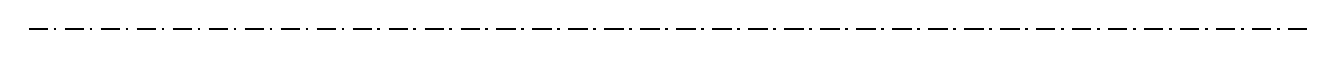
\begin{tikzpicture}
\draw [thick,dash pattern={on 7pt off 2pt on 1pt off 3pt}] (0,0) -- (16.3,0);
\end{tikzpicture}

{\bf Bachelor of Engineering} \hfill {\em 2013 - 2017} 
\\  \textit{\bf Southern University of Science and Technology, CN} \hfill 3.6/4.0
\\ \textit{Department of Computer Science and Engineering}

%Minor in Linguistics \smallskip \\
%Member of Eta Kappwta Nu \\
%Member of Upsilon Pi Epsilon \\
\end{rSection}
%----------------------------------------------------------------------------------------
%	TECHNICAL STRENGTHS SECTION
%----------------------------------------------------------------------------------------

\begin{rSection}{RESEARCH Keywords}
   \begin{itemize}
   \itemsep-0.4em 
    \item \textit{Computer Vision} and \textit{Natural Language Processing};
    % \item \textit{Weak/Un-Supervised Representation Learning;}
    \item \textit{Vision and Language Pre-training and Knowledge Distillation}
    \item \textit{VL tasks: Image/Video Captioning, Retrieval, VQA}, and \textit{Grounding.}
    % \item \textit{Commonsense Knowledge based Video Understanding.}

    \end{itemize}
\end{rSection}



\begin{rSection}{Previous Experiences}

% \begin{rSubsection}{Research Intern@ Microsoft Research, Redmond}\hfill{Summer, 2021.}{ Vision and Language Pre-training, \\Collaborators: \hfill\textbf{Jianfeng Wang, Zhe Gan, Lijuan Wang, Zicheng Liu}}
% \item{Knowledge Distillation on vision and language model, i.e., DistillVLM.}
% \end{rSubsection}

\begin{rSubsection}{Research Intern@ Microsoft Cloud \& AI, Redmond}\hfill{\textbf{Jan, 2021. - Sep, 2021}}{ VL Pre-training, Knowledge Distillation \\Collaborators: \hfill\textbf{Jianfeng Wang, Zhe Gan, Lijuan Wang, Zicheng Liu}}
\item{Vision and Language Model Pre-training, Compression via Knowledge Distillation, etc. }
\end{rSubsection}

\begin{rSubsection}{Research Intern@ Microsoft Research, Redmond}\hfill{\textbf{May, 2020. - Sep, 2020}}{ Self-supervised Representation Learning \\Collaborators: \hfill \textbf{Jianfeng Wang, Lei Zhang, Lijuan Wang, Zicheng Liu}}
\item{Self-supervised Representation Learning \& Knowledge Distillation on large scale visual data.}
\end{rSubsection}

\begin{rSubsection}{Visiting Student@ MMlab of Chinese Academy of Sciences}\hfill{\textbf{Sep 2016 - Feb 2017}}{Face Recognition, \textbf{\textit{Yu Qiao, Zhifeng Li}}}{}
\item Deep face recognition; Contrastive loss design.
\end{rSubsection}

\begin{rSubsection}{Visiting Student@ University of California, Irvine}\hfill{\textbf{June 2016 - Sep 2016}}{Deep learning, Biomedical Image processing,  \textbf{\textit{Pierre Baldi}}}{}
\item Bio-Medical image processing; Object segmentation and detection.
\end{rSubsection} 

\end{rSection}

\begin{rSection}{Selected Publications \& Pre-prints} 
% \itemsep -2pt
{\small *: equal contribution} 
\begin{enumerate}
%   \itemsep-0.25em 
    
    % \item\href{}{\textit{``Exploreing the Vision Transformer based Image Captioner through the Lens of Multi-Scale''}}{\\ \textbf{Zhiyuan Fang}, Jianfeng Wang, Zhe Gan, Xiaowei Hu, Lijuan Wang, Yezhou Yang, Zicheng Liu. (Aug, 2021) }
        
    \item\href{https://arxiv.org/abs/2104.02096}{\textit{``Compression Visual-linguistic Model via Knowledge Distillation.''}}{ \textbf{Zhiyuan Fang}, Jianfeng Wang, Xiaowei Hu, Lijuan Wang, Yezhou Yang, Zicheng Liu. (International Conference on Computer Vision (ICCV), 2021) }
    
    % \item \href{}{Arnav Chakravarthy, \textbf{Zhiyuan Fang}, Yezhou Yang \textit{``Tragedy Plus Time: Capturing Human Unintended Activities fromWeakly-Labeled Videos''}, March, 2021 (under review)}
    
    % \item \href{}{Yiran Luo, \textbf{Zhiyuan Fang}, Yezhou Yang, Chitta Baral, \textit{``Action-conditioned Structured Event Learning from Videos''}, March, 2021 (under review)}
        
    % \item \href{}{Huiliang Shao$^*$, \textbf{Zhiyuan Fang}$^*$, Yezhou Yang, \textit{``CAVAN: Commonsense Knowledge Anchored Video Captioning''}, Nov, 2020 (under review)}
    
    \item \href{https://arxiv.org/abs/2101.04731}{\textit{``SEED: Self-Supervised Distillation for Visual Representation.''}}{\textbf{{Zhiyuan Fang}}, Jianfeng Wang, Lijuan Wang, Lei Zhang, Yezhou Yang, Zicheng Liu,(International Conference on Representation Learning (ICLR), May, 2021)}
    
    % \item \href{}{\textbf{{Zhiyuan Fang}}, Shu Kong, Zhe Wang, Charless Fowlkes, and Yezhou Yang, \textit{``Temporal
    % language grounding with referring attention and weak supervision''}, April, 2020 (arXiv:2006.11747)}
    
    \item \href{https://arxiv.org/pdf/2003.05162.pdf}{\textit{``Video2commonsense (v2c): Learning to transform video scenes to commonsense knowledge.''}}{\textbf{{Zhiyuan Fang}}, {Tejas Gokhale}, Chitta Baral, and Yezhou Yang, ({\textit{Empirical Methods in Natural Language Processing (EMNLP)}}, Long Paper, 2020)}
    
    \item \href{https://arxiv.org/abs/2005.07327}{\textit{``ViTAA: Visual-Textual Attributes Alignment in Person Search by Natural Language.''}} {Zhe Wang$^*$, \textbf{{Zhiyuan Fang$^*$}}, Jun Wang and Y Yang, ({\textit{European Conference on Computer Vision (ECCV)}}, 2020)}
    
    \item \href{https://openaccess.thecvf.com/content_CVPR_2019/papers/Fang_Modularized_Textual_Grounding_for_Counterfactual_Resilience_CVPR_2019_paper.pdf}{\textit{``Modularized Textual Grounding for Counterfactual Resilience.''}}{\textbf{Zhiyuan Fang}, Shu Kong, Charless Fowlkes, Yezhou Yang, ({Conference on Computer Vision and Pattern Recognition (CVPR)}, 2019)}
    
    % \item \href{}{Tejas Gokhale, Shalaija Sampat, \textbf{{Zhiyuan Fang}}, Yezhou Yang and Chitta Baral, \textit{``Blocksworld Revisited: Learning and Reasoning to Generate Event-Sequences from Image Pairs'' ({CVPR workshop on Language and Vision, 2019})}}
    
    \item \href{https://arxiv.org/abs/1805.00545} {\textit{``Weakly Supervised Attention Learning for Textual Phrases Grounding.''}} {\textbf{{Zhiyuan Fang}}, Shu Kong, Tianshu Yu, Yezhou Yang, \textit{({CVPR Vision and Language Workshop}, 2018)}}
    
    \item \href{https://arxiv.org/abs/1611.08976} {\textit{``Range Loss for Deep Face Recognition with Long-tail.''}}{Xiao Zhang, \textbf{{Zhiyuan Fang}}, Yandong Wen, Zhifeng Li, Qiao Yu, ({\textit{International Conference on Computer Vision (ICCV)}}, 2017)}
    
    \item \href{http://www.sciencedirect.com/science/article/pii/S0010482517300793} {\textit{``A Multi-resolution Analysis Approach for Spinal Metastasis Detection using Siamese Neural Network.''}} {Juan Wang, \textbf{{Zhiyuan Fang}}, Ning Lang,  Huishu Yuan, Lydia Su,  Pierre Baldi,
    \textit{{(Computers in Biology and Medicine}, 2017)}}(Honor Paper, 5\%)

    % \item \href{http://ieeexplore.ieee.org/stamp/stamp.jsp?arnumber=7509785}{\textbf{{Zhiyuan Fang}}, Lingqi Zhang, Kun Chen,  \textit{``A Behavior Mining Based Hybrid Recommender System''}}, {(IEEE, {\textit{International Conference on Big Data Analysis}}, 2016)}
\end{enumerate}


\end{rSection}



\begin{rSection}{Teaching Associative:}

{\textit{FIN 330: Data Mining and Data Analysis }}\hfill \textit{SUSTech, 2017 Spring}\\
{\textit{CSE 205: Object Oriented Programming}}\hfill \textit{ASU, 2017 Fall, 2018 Spring}\\
{\textit{CSE 310: Data Structure and Algorithm}}\hfill \textit{ASU, 2017 Fall, 2018 Fall, 2021 Fall}\\
{\textit{CSE 571: Artificial Intelligence}}\hfill \textit{Coursera-ASU, 2019 Spring}\\
\end{rSection}
%----------------------------------------------------------------------------------------
\begin{rSection}{Awards}
\itab{\textit{Outstanding Reviewer }}\hfill{\textit{British Machine and Vision Conference, 2019}}\\
\itab{\textit{Fulton Engineering Graduate Fellowship }}\hfill{\textit{Ira Fulton School of Engineering, 2019}}\\
\itab{\textit{Honor Paper Award (5\%)}}\hfill{\textit{Computers in Biology and Medicine, 2018}}\\
% \itab{\textit{Bachelor Thesis Award (5\%)}}\hfill{\textit{SUSTech, 2017}}\\
% \itab{\textit{Excellent Oral Presentation Award}}\hfill{\textit{ICBDA, IEEE, 2016}}\\

\end{rSection}


%----------------------------------------------------------------------------------------
\begin{rSection}{Academic Services}
\itab{\textbf{Journal reviewer:}}\hfill{\textit{TIP, IEEE; Patter Recognition, Elsevier; TCSVT, IEEE}}\\
\itab{\textbf{Conference Committee:}} 
% \hfill{\textit{BIBE, IEEE, 2018}}\\
% \strut\hfill{\textit{CSAE, 2018}}\\
\strut\hfill{\textit{{Neurips}, {CVPR}, {ICCV}, {ECCV}, {AAAI}, {ICLR}, {BMVC}, {ICRA}, etc.}}\\
% \itab{\textbf{Emergency reviewer:}} 
% \strut\hfill{\textit{{CVPR 2020}}}\\
\end{rSection}

%----------------------------------------------------------------------------------------
% \begin{rSection}{Professional Skills}
% \itab{\textbf{Platforms:}}\hfill{\textit{Azure ML, AWS EC2; Docker}}\\
% \itab{\textbf{Programming languages:}}\hfill{\textit{Python, Java, R,, LaTex, HTML, etc}}\\
% \itab{\textbf{Framework \& Systems:}}\hfill{\textit{Ubuntu, Pytorch, Keras and etc}}\\
% \itab{\textbf{Languages:}}\hfill{\textit{Mandarin, English}}
% \end{rSection}


%----------------------------------------------------------------------------------------
\begin{rSection}{Referees}
\textbf{\textit{Yezhou Yang}} (Ph.D. Advisor) \hspace{27mm} {\textbf{\textit{Shu Kong}}}\\
Assistant Professor, Arizona State University \hfill  Postdoc Researcher, Carnegie Mellon University\\
% \textbf{Address:} \textit{699 S. Mill Ave. Tempe, AZ} \hspace{14.mm} \textbf{Address:} \textit{5000 Forbes Ave, Pittsburgh, PA} \\
% \textbf{Tel:} 301-661-3865   \hspace{4.4cm} \textbf{Tel:} 301-661-3865 \\
\textbf{Email: }\url{yz.yang@asu.edu} \hspace{36.7mm} \textbf{Email: } \url{shuk@andew.cmu.edu} \\

\textbf{\textit{Tianshu Yu}} \\
Assist. Professor, Chinese University of Hong Kong \\
\textbf{Email: }\url{tianshuy@asu.edu} 

\end{rSection}

\end{document}
